\chapter{Koblitz curves}\label{sec:koblitz}

Koblitz curves $E_a: y^2+xy=x^3+ax^2+1$ over $\FF_{2^n}$, $a\in\{0,1\}$, carry
the Frobenius endomorphism $\tau$, which acts on the prime-order subgroup as
a known scalar $\lambda$; ECC2K-130 is the $a=0$, $n=131$ member. They were
the programme's main family: the compact-orbit producer, the $n=83$
campaign, leaderboard Table~A and the ECC2K-130 cost model all live here.
Random and prime-degree binary curves without $\tau$ are in
\S\ref{sec:binary}, and the Weil-descent degree studies that price
ECC2K-130's algebraic route are there too, because their systems use random
subspaces rather than Frobenius structure. Every study in this section is
listed in the programme record~\cite{icprogram2026}.

\section{Frobenius-invariant and compact-orbit bases}

The Koblitz implementation (\art{src/cryptanalysis/koblitz_index_calculus.rs})
builds GGMP's invariant base from the linearised polynomial of a factor of
$x^n-1$, checks $\pi(\Fb)=\Fb$ point by point, rewrites each relation into
orbit columns with known $\lambda^k$ weights, and solves the
cofactor-corrected system $h a+hbd\equiv\sum\lambda^{k_i}x_{o_i}$. On
small fields the orbit collapse is as predicted: $\abs\Fb/\#\text{orbits}$
of $7.86$, $10.89$, $12.96$ at $n=9,11,13$ for relations and
$61.7$--$168.0$ for linear algebra, against rho's $4.24$--$5.10$
(\art{RESEARCH_KOBLITZ_INDEX_CALCULUS.md}). Because $\ell=\operatorname{ord}_n(2)$
fixes the invariant base's size, the programme moved to bases sized to the
instance: divisor bases, SAT-optimised bases, a rank-guided base at $n=53$
(220 orbits, a complete implicit $\Sem5$ formula of 22{,}887 clauses), and
finally the \emph{compact signed-Frobenius orbit} base, which stores one
representative per orbit and no pair table
(\art{docs/ic/COMPACT_ORBIT_PRODUCER.md}). In the ecbench factor-base
suite it is the best measured Koblitz construction: $S=9.114$ at $n=17$
($272$ points, 8 columns), $9.985\times$ matched signed-Frobenius rho,
against full orbit $18.7\times$ and subspace bases $47\times$
(\art{research/ecbench_frontier_20261013/}).

\section{The oracle sequence}

The binary oracle went through SAT (XOR-native CDCL after Trimoska et
al.~\cite{trimoska2020}; decides the $n=19$, $\ell=6$ corpus but does not
scale), matrix F4 (whose refutation range was the real frontier),
pairs-and-solve for $\Sem4$ (validated to $n=21$, $\ell=7$, still
$O(2^{2\ell})$), meet-in-the-middle pair tables, inherited F4 and F6-IC
(\S\ref{sec:groebner}), and root-finding engines (\S\ref{sec:rootfinding}).
The boundary ledger's current Koblitz decomposition record is an $n=31$,
$m=2$ F4 cell with an exact block-6 M4RI acceleration; at $n=53$ an exact
Frobenius-orbit $\Sem5$ compression removes the coordinate ROM but every
unrestricted solver arm remains \textsc{unknown}.

The September toy studies that fed this sequence are catalogued as
campaigns. At $n=13$ and $n=19$, rotated subspace bases covered $1{,}591$ of
$2{,}003$ targets with five spaces against $61$ with one, and joint rank
recovered $58/64$ targets against $29/64$, without passing a 10\% yield
gate at $n=19$ (\art{research/notes/ecc2k130/}, clusters
``rotated-n13'' and ``rotated-n19''). Finite-fibre $\Sem3$ semantics were
proved exact and an $O$-aware CNF made $252.7\times$ smaller at $n=13$, but
no existing solver interface was admitted as an arm; three SAT engines
decided 5 satisfiable and 27 unsatisfiable targets at $n=13$, with the five
negatives DRAT-certified. At $n=131$ a symbolic full-point DAG replayed a
single-edge DIMACS instance but could not be admitted past the 64-bit
ceiling, and the exact Frobenius census of the balanced $(m,d)=(10,13)$
rotated base has $1{,}048{,}134$ columns, the only shape with as many columns
as the field. A frozen test of the Frobenius quotient found that toy fields
saturate and so test nothing; an independent SAT reproduction solved
$n=13$ and none of four planted targets at $n=19$ in 1{,}200\,s
(\art{research/frobenius_quotient_sat_20260930/}). At $n=13$ the
presentation of the curve does not matter: yield spread is explained by
cofactor balance (correlation $0.850$) and there is no curve effect at
$n=19$ (intraclass correlation $\le0.006$;
\art{research/koblitz-isogeny/}).

\section{Against a stronger rho: the September reversals}\label{sec:koblitz-strong}

Three September results that put Koblitz index calculus at or below rho
were reversed when rho was strengthened, which is why every later row is
quoted against the strongest available rho
(\S\ref{sec:corrections}). Table~\ref{tab:prog_koblitz-reversals} gives
each result as recorded and against the stronger rho.

\begin{table}[t]
\centering\small
\begin{tabular}{@{}llllr@{}}
\toprule
Result & Case & Measure & Recorded & Stronger rho \\
\midrule
Tournament & $n=43$, $a=1$, best & retired instr. & $0.5347$ & \\
 & $n=43$, $a=1$, triple table & & $0.409$ & \\
 & five cells$^{e}$ & & & $1.19$--$2.88\times$ \\
\addlinespace
Orbit DLP & $n=53$, 1{,}024 targets & retired instr. & $0.2403$ & \\
 & four rungs & & & $0.240\to0.317\to1.294\to1.923$ \\
 & sweep, $n=37$ & & & $0.794$ \\
 & sweep, $n=41$ & & & $1.520$ \\
 & sweep, $n=53$ & & & $1.923$ \\
 & sweep, $n=61$ & & & $2.297$ \\
 & single target & & $0.8392$$^{a}$ & $44.0\times$ $[39.4,45.4]$ \\
\addlinespace
Compact orbit & $n=41$, $L=1{,}024$ & corrected rho & $0.309\times$ & \\
 & $n=37$, $L=1{,}024$ & 32-walk rho$^{b}$ & & $2.081$ \\
 & $n=53$, $L=1{,}024$ & & & $3.086$ \\
 & $n=41$, $L=1{,}024$ & cold CPU$^{c}$ & & $1.314$ \\
 & $n=53$, $L=1$ & & & $22.675$ \\
 & $n=37$, $L=1{,}024$ & instructions$^{d}$ & & $0.5165\times$ \\
 & $n=41$, $L=1{,}024$ & & & $0.6221\times$ \\
\bottomrule
\end{tabular}
\caption[]{IC/rho of the three September results as first recorded and
against a strengthened rho. Tournament (15 September): IC against a worker
rho's retired instructions; giving rho the index calculus's own canonical
form made rho win all five cells
(\art{research/ic_triple_counted_20260923/}; the tournament README,
\art{research/ic_candidate_tournament_20260915/}, carries no correction
note). Orbit DLP: the recorded rho used software carry-less multiplication
on x86-64; rho was strengthened in four rungs, then the preregistered sweep
read rising with $n$
(\art{research/notes/index-calculus/RESEARCH_STRONG_RHO_LADDER_20260929.md});
$^{a}$the selected-panel crossover withdrawn by the direct arm's cost
against a strong single-target rho
(\art{research/notes/index-calculus/RESEARCH_SINGLE_TARGET_STRONG_RHO_N53_20260930.md}).
Compact orbit: the recorded value is a point panel;
$^{b}$a 32-walk batched-inversion normal-basis rho
(\art{research/notes/ecc2k130/compact_orbit_strong_rho_20260929/RESULT.md});
$^{c}$compact/rho CPU of the orbit-disjoint cold confirmation, which ended
with six eligible no-gos
(\art{research/notes/ecc2k130/disjoint_cold_v2_outcome_20261001/RESULT.md});
$^{d}$batched compact IC
(\art{research/notes/ecc2k130/compact_ir_ledger_20260930/RESULT.md}).
$^{e}$Rho given the index calculus's own canonical form.}
\label{tab:prog_koblitz-reversals}
\end{table}

Batched compact IC does use fewer instructions than rho while its cold CPU
stays above rho, a gap traced to memory behaviour. Some sixty notes on S3
batch inversion, swap quotients, Bloom prefilters, window screens and $K$
grids each moved a constant and none crossed rho (cluster
``compact-orbit-cold'').
The boundary ledger of the same weeks reached the same place from the other
side. Re-pricing every row against a matched negation rho raised the vs-rho
ratios $2.1$--$6.5\times$ (\art{research/ic_rho_reference_20260923/}); the
best batch row was $4.86\times$ $[4.21,5.55]$ at $r=2^{39}$, and a page
$r^{1/6}$ law was falsified at the small end
(\art{research/ic_exponent_20260926/}); single-target online IC beat
table-less rho at all six sizes ($8.84$--$17.5\times$) while cold rho won at
all six ($1.98$--$31.6\times$; \art{research/ic_single_target_20260930/}).
At $n=37$ in ecbench the cold IC/rho was $3.64\times$ in instructions and
$13.6\times$ $[10.6,18.7]$ in counted $S$, and the $n=37$ parameters did not
transfer to $n=41$ or $n=53$
(\art{research/ecbench_n37_shared_rank_20261004/},
\art{research/ecbench_n41_n53_shared_rank_20261005/}). An $m=4$ exponent
audit measured a cost slope of $0.985$--$1.060$ bits per unit of $n$ at
$n\le19$, against the $0.25$ the lead needed
(\art{research/ic_m4_exponent_audit_20260928/}).

\paragraph{Other Koblitz lines.} The remaining Koblitz campaigns moved
constants inside index calculus and are catalogued in
the programme record~\cite{icprogram2026}. Instruction-level rounds on the Gröbner stage
left the whole relation log at $964\times$ rho on $K_0$ over $\FF_{2^{13}}$
(\art{research/groebner_instructions_20260925/}); a September autolab
campaign cut cold instructions by $47.7\%$ and left the candidate at
$4.98\times$ matched rho's instructions (\art{research/ic_autolab_next30_20260915/});
at $n=37$ a full-rank compact-orbit gate passed with IC at $22.6\times$ rho
(\art{research/notes/ecc2k130/full_rank_compact_orbit_ic_20261003/RESULT.md}).
Pipeline kernels gave laned canonical keys $1.09$--$1.31\times$
(\art{research/canon_laned_keys_20261008/}), u64 root batching
$3.26\times$ whole-process wall (rank cell corrected to $2.47\times$), and
aimed gathering $1.037\times$ set-up (\art{research/ic_aimed_gather_20261023/}).
Transporting a base through ECC2K-130's degree-263 and degree-7 isogenies
was built and certified, but on toy fields the transported and descendant
bases cost $3.6$--$4.0\times$ the original
(\art{research/ecc2k130_factor_base_pilot_20260924/}); and $\tau$-adic
known-scalar arithmetic is $0.413$ of the binary cost at $m=131$ with no
measured rho benefit
(\art{research/notes/ecc2k130/tau_adic_arithmetic_20260929/README.md}).
On the rho side, GPU iteration redesigns for the ECC2K-130 walk did not
beat the shipping distinguished-point walk
(\art{research/ecc2k130_iteration_redesign_20261012/},
\art{research/dp32_sigma_table_20261012/}).

\section{The one-target online ladder}

The ledger's primary \texttt{vs\_rho} question is: with reusable IC
preparation already done, how long does one unseen public target take,
against rho with the automorphism discount on the same point? The ladder
(Figure~\ref{fig:online}) is in Table~\ref{tab:prog_koblitz-ladder}.

\begin{table}[t]
\centering\small
\begin{tabular}{@{}rlrrlrl@{}}
\toprule
$n$ & Base & Columns & Points & Memory & Rho/IC online & Status \\
\midrule
53 & shared-log$^{a}$ & & & 9.34\,GB & & \\
61 & compact orbit & 600 & 73{,}200 & 2.73\,GB & $124.85\times$ & exploratory$^{b}$ \\
71 & & & 85{,}200 & & $2{,}864.1\times$ & exploratory$^{c}$ \\
73 & & & 87{,}600 & & $1{,}189.7\times$ & exploratory$^{d}$ \\
83 & $a=1$ & & & & $8.2\times$ & exploratory$^{e}$ \\
\addlinespace
\textbf{61} & orbit, $a=0$ & $K=500$ & $61{,}000$ & & $13.94\times$ $[9.81,19.13]$ & admitted$^{f}$ \\
 & & & & & $12.87\times$ $[7.30,19.08]$ & admitted$^{g}$ \\
\bottomrule
\end{tabular}
\caption[]{The one-target online ladder: rho online time over IC online
time on the same point, reusable IC preparation excluded; peak memory where
recorded (peak RSS at $n=53$). $^{a}$Guided shared-log precompute with an
explicit pair table; earlier, a 1{,}024-target shared-log batch beat batched rho
in all 15 paired blocks (secondary, multi-target). $^{b}$Fresh
reproduction. $^{c}$First rung past 64-bit packing (u128 words); median of three
repeats of one point. $^{d}$The guided-rank precompute took 5.1\,h at
57--70 million probes per relation. $^{e}$IC online 5.6--7.9\,s against
rho 43--71\,s; re-measured below. $^{f}$Admitted 12 October: 64 fresh
public one-target workloads per host, identical candidate manifest on two
hosts; median online speed-up with 95\% interval; pinned x86\_64,
claim-check 64/64. $^{g}$The same, unpinned arm64.}
\label{tab:prog_koblitz-ladder}
\end{table}

Re-measured on 12 October against a default strong rho on five repeats of
the same target, the $n=83$, $a=1$ IC was \emph{slower} online,
$1.382\times$ $[1.036,1.882]$, and $218.0\times$ rho in fresh-process wall
time (\art{research/n83_evaluation_20261012/}); the later dense-root
reading of $18.5\times$ is in \S\ref{sec:n83}. For the admitted $n=61$
point, set-up of about 28\,s is outside the window; with it charged, IC
costs a median $83.4\times$ rho.

\begin{figure}[t]
\centering
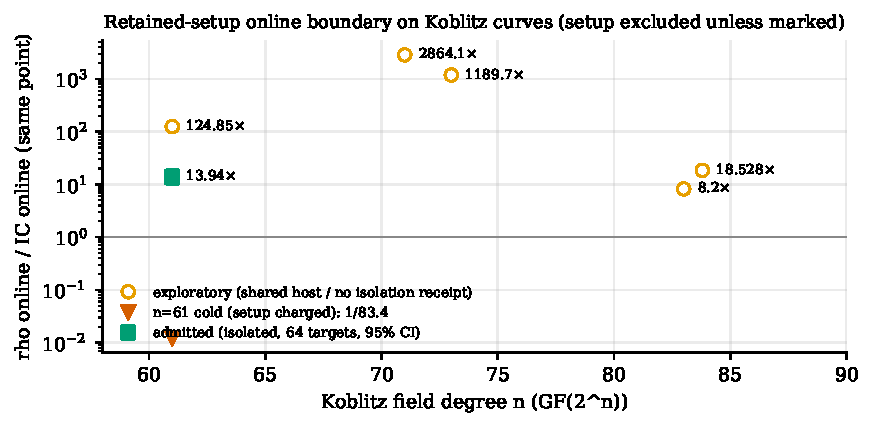
\includegraphics[width=\linewidth]{figures/fig-koblitz-online.pdf}
\caption[]{Rho online time over IC online time on the identical public point,
reusable IC preparation excluded. Open circles: exploratory (verified
answers, no qualifying isolation receipt; three repeats of one point or a
single point). Filled square: the admitted 64-workload panel with its 95\%
bootstrap interval. Triangle: the same $n=61$ candidate with set-up
charged (cold). Sources: \art{docs/ic/boundary_targets.json},
\art{docs/ic/PLAN_IC_ACCOUNTING_FIXES_20261007.md},
\art{research/n83_dense_root_20261013/}.}
\label{fig:online}
\end{figure}

The exploratory ratios are large and irregular because a one-point online
window measures the luck of one relation search against one rho walk; the
admitted panel's range over 64 workloads is $1.06$--$648.6\times$. The
admitted point is a constant-factor online result at $n=61$ (47-bit
subgroup) with preparation retained; it is not a cold result, not a
scaling law, and not an asymptotic claim.

\emph{Retired as an index-calculus win (14 October).} Every rung of this
ladder compares index calculus with a retained table against rho with
none. Given a distinguished-point table of equal or smaller size,
Bernstein--Lange preprocessing rho~\cite{bl2012} is $53$--$317\times$
faster online than the compact-orbit arm on the same 64 targets at $n=41$,
53 and 61 (\S\ref{sec:ladder}). At $n=83$ (\S\ref{sec:n83}) rho with a
table matched to the index calculus's set-up time or memory won every pair
that was run. The ladder therefore measures what a table buys, and generic
rho buys more per byte. The validation sweep later found
\art{docs/ic/BOUNDARY_TARGETS.md} still printing the $13.94\times$ as a
win; it is superseded
(\art{research/validation_sweep_20261019/B-benchmarks/VERDICT_TABLE.md}).

\section{The $n=83$ campaign}\label{sec:n83}

Degree 83 was the programme's largest Koblitz target with a working
pipeline: 145 study directories between 4 and 21 October
(the programme record~\cite{icprogram2026}, clusters beginning ``n83'' and ``f6-n83'').
In order:
\begin{itemize}
\item \emph{F6 micro-studies, 4--5 October} (24 directories, almost all on
  the $a=0$ curve). They kept kernel gains (queries up to $2.998\times$
  faster, resident memory $-52\%$) and shrank SAT encodings, but every
  ordinary solve timed out; four-summand coverage was at most
  $4.662\cdot10^{-12}$ of the subgroup and no natural relation was found.
  On the 81-bit $a=0$ gate curve, SAT and XCNF decompositions succeed only
  with a known witness, and the prebuilt-base question is an open problem
  record.
\item \emph{The $a=1$ point, 7--12 October.} The archived K600 point read
  $8.2\times$ online and was re-measured slower (above).
\item \emph{Root-index capacity, 13--16 October} (25 directories). Root-index
  layouts grew the $a=1$ base from K512 ($84{,}992$ points) to K3596
  ($596{,}936$ points) within 14\,GiB. The dense root index cut probes per
  relation from $300{,}021.9$ to $169{,}069.8$ (K1500 to K1798; paired
  difference $130{,}952$ $[52{,}058,209{,}990]$), a within-IC result that
  stands; its one-point online $18.528\times$ is retired
  (\art{research/n83_dense_root_20261013/}).
\item \emph{Factor-base selection, 14--16 October} (56 directories). Root4,
  root11 and root21 layouts, Bloom filters, sparse and canonical variants
  and $K$ screens from 100 to 20{,}000 points selected within index calculus;
  the best means are about 26--29\,ms online (K3425, K3450, K3500), and
  many screens end \textsc{bounded\_unknown}. A three-hash 512\,MiB Bloom
  filter cut a K3300 online mean from $34.77$ to $31.32$\,ms
  (\art{research/n83_root11_bloom_results_20261015/}); a K3350 win of
  $7.18\%$ did not replicate.
\item \emph{Tier-1 online readings, 14--16 October} (14 directories): median
  rho/IC of $54.1$, $210.3$, $113.0$, $104.2$, $35.1$, $413.3$ (one point)
  and $208.7\times$ (K3072, five fresh points, $[38.3,2{,}510]$;
  \art{research/n83_tier1_online_20261016/}), all against a rho with no
  table and with set-up excluded.
\item \emph{The control, 16 October.} Bernstein--Lange rho given a
  distinguished-point table matched to the index calculus's set-up time or
  memory was faster online in every pair run: IC/rho $3.74$
  $[2.65,11.05]$ (K3300, time-matched), $40.61$ (K3300, memory-matched),
  and $81.5$--$395.5$ (K600)
  (\art{research/20261016-n83-precomputed-rho-control/}). Only the K3300 and
  K600 bases were paired; the K3072 reading was not, so its retirement rests
  on the same mechanism rather than on its own measurement. The validation
  sweep and the ledger audit retired all the online readings on 19--20
  October.
\item \emph{Cold, 16--21 October} (11 directories). The cold one-target
  process fell from about 150\,s (K1024) to $119.8$\,s (K1120, holdout) and
  $113.8$\,s (K1107; \art{research/n83_cold_base_confirm_20261021/}), against
  a rho online time of about 2.2--2.6\,s on the same hosts. No matched cold
  rho was run, so no cold ratio is admitted; the hosted single-target
  benchmark's $133.7\times$ is the nearest cold figure
  (\art{benchmarks/20261014-n71-n83-hosted-single-target/}).
\item \emph{A second pipeline in \texttt{cryptanalysis}} (K600, $a=1$;
  \cite{icprogram2026}). A Tier~1 ratchet of rank-probe, closure,
  index-build and rank-finder changes brought its latest row to $3.92\times$
  a tuned rho end to end, cold, and $0.093\times$ online with set-up
  excluded (\art{ca:experiments/koblitz-n83-rankfinder-20261021/README.md}).
  The study's own limits apply: one run on one host class, a point estimate
  with no interval, wall time, factor-base construction charged to no arm (so
  the cold cost is a lower bound), no computable band, and gaps that are not
  comparable across runs (the same producer read $4.42\times$ on another host).
  Against Bernstein--Lange rho with equal advice its online time is
  $22.55\times$ $[16.23,31.44]$ worse
  (\art{ca:experiments/koblitz-n83-bl-rankprobe-20261019/}). It is the
  closest cold Koblitz figure at $n=83$ and is still above rho; the two
  pipelines' numbers are not comparable with each other.
\end{itemize}
The open pull requests at the time of writing include further $n=83$ work
($m=4$ queries on a retained 16{,}627-column base, AWS replays, shared-binary
panels); none is on \texttt{main} (the programme record~\cite{icprogram2026}).

\section{Leaderboard Table A: the Koblitz rules}\label{sec:tablea}

Table~A of \art{docs/ic/LEADERBOARD.md} prices one unseen public target on
Koblitz curves at $n=41$--$61$ ($\log_2r=36.6$--$47.2$), cold, against rho on
the same point. Its history is a sequence of rules, each a pipeline baseline
plus a rho reference (\art{research/ic_tool_program/}).
Table~\ref{tab:prog_koblitz-tablea} lists the rules and the pipeline
baselines.

\begin{table}[t]
\centering\small
\begin{tabular}{@{}llr>{\raggedright\arraybackslash}p{0.3\linewidth}@{}}
\toprule
\multicolumn{4}{@{}l}{(a) Rules: cold IC/rho on one unseen public target} \\
\midrule
Rule & Date & IC/rho, cold & Status \\
\midrule
v3 & & $5.23$--$21\times$ & printed in Table~A; unvalidated (pre-gate) \\
v6 & & $3.78$--$12.06\times$ & rho reference $0.57$--$0.85$ of strong walk$^{a}$ \\
v7 & & $3.43$--$11.51\times$ & rho reference $0.57$--$0.85$ of strong walk$^{a}$ \\
v8 & 19 October & $4.67$ $[4.34,5.07]$ to $18.07$ $[15.98,20.58]\times$ & matched GFNI rho; archived as incomplete$^{b}$ \\
v4 recipe & 24 October & $9.9$--$43\times$ & validation file withheld$^{c}$ \\
\bottomrule
\addlinespace
\multicolumn{4}{@{}l}{(b) Pipeline baselines, 16--17 October: cold speed-up} \\
\midrule
Baseline & Change & Cheaper cold & \\
\midrule
v4 & head-of-main & & \\
v5 & scan-key & $1.20$--$1.24\times$ & \\
v6 & scan-fold & $1.33$--$1.40\times$ & \\
v7 & build streams & $1.07$--$1.13\times$ & \\
v8 & admitted prefetch & $1.06\times$ & \\
v4$\to$v8 & together & $1.90$--$1.98\times$ & \\
\bottomrule
\end{tabular}
\caption[]{Leaderboard Table~A, Koblitz $n=41$--$61$. (a)~Each rule's
cold IC/rho range over its sizes, against rho on the same point (rules v6
and v7: \art{benchmarks/20261016-ic-rule-v7/}; v8:
\art{benchmarks/20261019-ic-matched-rho-v8/}; v4 recipe:
\S\ref{sec:ladder3}). $^{a}$Per step, so the distance was understated.
$^{b}$$1.30$--$1.58\times$ the v7 control, fitted slope $0.168$ per $\ln r$;
its row is listed although the run is archived as incomplete. $^{c}$A paired
retuning improved one size of six; rho is priced in the same process at the
canonical batched step, and the validation file is withheld because that
reference may not be the strongest, so it is not an admitted row either.
(b)~Each baseline's recorded speed-up, and the combined cold factor over
v4 (\art{benchmarks/20261017-ic-r12-admitted-prefetch/}).}
\label{tab:prog_koblitz-tablea}
\end{table}

Under rules v6 and v7 cold rho was still faster at every size
(Table~\ref{tab:prog_koblitz-tablea}(a)). Seven further baseline candidates (prefetch gates,
filter slots, huge pages, a wider base) did not clear their rounds.
Table~C prices a 32-target batch on nine Koblitz curves ($\log_2 r=18$--$47.2$)
against batch rho on the same targets: $3.62$--$14.9\times$, a historical
diagnostic under the one-target rule. All nine failed the 24 October
validation gate, and Table~D, the Joux--Vitse historical study, is withheld.

The validation sweep found that Table~A understates its gap to rho by
$1.7$--$2.0\times$, and the 24 October validation gate did not check Table~A
(\art{research/ic_validation_gate_20261024/}). Rules v8 and v4 measure the
same sizes against differently built rho references and are kept apart
(Definition~\ref{def:domain}).

\section{ECC2K-130}\label{sec:ecc2k130}

ECC2K-130 is the $a=0$, $n=131$ member of the same family, with a 130-bit
prime subgroup and rho at about $2^{60.81}$ group operations. The compact
producer already solves $n=41,53,61,71,73$ of the family; about 300 notes
under \art{research/notes/ecc2k130/} price the routes to $n=131$ itself. No
route prices below rho.
Table~\ref{tab:prog_koblitz-ecc2k130} lists the priced algebraic routes.

\begin{table}[t]
\centering\small
\begin{tabular}{@{}llrr@{}}
\toprule
Route & Setting & Cost & Above rho \\
\midrule
Decomposition oracle & family bottom & $2^{132.58}$ & \\
 & Frobenius-orbit unions, $m=3$ & $2^{124.99}$ & $2^{64.18}$ times \\
\addlinespace
Relation sweep & best single relation, $m=4$ & & $+4.98$ bits \\
 & best honest $m=8$, Frobenius quotient & & $+13.59$ bits \\
\addlinespace
Linearisation & plain & & $70.19-b_{\max}$ bits \\
 & best bilinear XL, $\omega=2$ & & $71.82$ bits \\
 & same, $\omega=2.81$ & & $78.15$ bits \\
 & trilinear & & $87.16$ bits \\
\addlinespace
Weil descent & $m=3$, free oracle & $2^{68.58}$ & \\
 & $m=4$, degree 4 & $2^{68.43}$ & $+7.62$ bits$^{a}$ \\
 & $m=4$, degree 5, $w=1$ & $2^{71.13}$ & $+10.32$ bits \\
 & $m=4$, degree 5, $w=2$ & $2^{106.52}$ & $+45.71$ bits \\
 & $m=4$, hybrid guess & & $+8.43$ to $+58.27$ bits \\
\bottomrule
\end{tabular}
\caption[]{Priced algebraic routes to ECC2K-130. \emph{Setting}: the
variant priced ($m$ summands, $w$ as in the source, $\omega$ the
linear-algebra exponent); \emph{Cost}: the route's cost as recorded;
\emph{Above rho}: its distance to rho, as a factor or in bits. The
decomposition bottom needs a materialised base of $2^{44.53}$ points at
$m=3$; the $m=4$ single relation needs $2^{70.79}$ bytes; linearisation
gaps charge each Macaulay solve; the descent rows are in unconverted column
touches. $^{a}$Now contradicted. Sources:
\art{research/notes/ecc2k130/RESEARCH_ECC2K130_DECOMPOSITION_TARGETS.md},
\art{research/notes/ecc2k130/RESEARCH_ECC2K130_RELATION_SWEEPS.md},
\art{research/linearization_reach_20260930/},
\art{research/xl_bilinear_core_20261006/},
\art{research/xl_trilinear_t_unknown_20261006/},
\art{research/notes/ecc2k130/RESEARCH_ECC2K130_DESCENT_DEGREE.md}; the
hybrid guess is in \S\ref{sec:binary-descent}.}
\label{tab:prog_koblitz-ecc2k130}
\end{table}

\begin{itemize}
\item \emph{Extrapolating the producer.} The fitted probes-per-relation law
  $C\,r/(n^2K^2)$ with $C=1$ gives $1.1\cdot10^{18}$ core-years at $K=600$
  and $6.8\cdot10^{8}$ at $K=10^{12}$ columns
  (\art{RESEARCH_ECC2K130_IC_FEASIBILITY.md}, with the unexplained
  factor-of-5 gap in $C$ of \S\ref{sec:corrections}).
\item \emph{Decomposition oracles.} Decompositions exist, but no oracle
  finds one for less than $2^{131}$ per family; unions of Frobenius orbits
  lower the family's bottom but not to rho. Crossbred, RR-solver and WDSat
  oracles are engineering only: Crossbred is $0.023$ of F4's bit operations
  at $m=3$ but slower end to end, and the RR solvers' advantage over Semaev
  at $d=6$ is worthless against brute force.
\item \emph{Linearisation and Weil descent.} Neither reaches rho
  (Table~\ref{tab:prog_koblitz-ecc2k130}). The studies behind the descent
  rows, and the hybrid guess for the $m=4$ row, are in
  \S\ref{sec:binary-descent}.
\item \emph{Covers.} Over $\FF_{2^{131}}$ every ordinary curve has GHS
  magic number 1 or 131, so GHS descends ECC2K-130 to genus 1 (a zero map on
  the subgroup) or to genus about $2^{130}$, and the Hess--Menezes--Teske walk
  has nowhere to land. One question is open: $\langle G\rangle$ is the group
  of a simple 130-dimensional abelian variety, and if that variety were
  isogenous to a Jacobian with an evaluable isogeny, index calculus on the
  genus-130 curve would cost $2^{37.17}$, $2^{23.64}$ times \emph{less} than
  rho; no such curve is known, the Torelli codimension at genus 130 is
  8{,}128, CM constructions with prescribed Frobenius stop at genus 3, and the
  largest published Weil-descent discrete logarithm is at genus 31 over
  $\FF_{32}$ (\S\ref{sec:transfer})
  (\art{research/notes/ecc2k130/RESEARCH_ECC2K130_HYPERELLIPTIC.md}, with the
  magic-number correction of
  \art{docs/audits/GHS_MAGIC_NUMBER_MMT_CORRECTION_20261013.md}). The
  $N=130$ counterfactual is genus 255 at a modelled $2^{55.60}$ against rho's
  $2^{60.31}$, and measuring one relation trial turns that margin negative
  (\S\ref{sec:ladder3}). The best explicit curve construction reaches genus
  $2^{28.92}$
  (\art{research/notes/ecc2k130/RESEARCH_ECC2K130_CURVE_CONSTRUCTION.md}).
  The isogeny class has 262 curves of conductor gap 263 and no measured
  level effect (\S\ref{sec:transfer}); rho on the degree-263 leaves keeps
  only the negation map, an $11.45\times$ penalty
  (\art{research/notes/ecc2k130/isogeny_rho_speed_20260930/}).
\item \emph{Rho itself.} The separate GPU rho estimate is about 4.3 RTX PRO
  6000 card-years (\art{paper/ecc2k130/}); on one CPU core the ECC2K-130
  client walks 13.2 million steps per second
  (\art{research/certicom131_rho_ic_bench_20261022/}). Signed $\sigma$ steps
  cut modelled GPU time to $0.961$--$0.970$
  (\art{benchmarks/20261014-ecc2k130-signed-sigma/}).
\end{itemize}
Index calculus is not a route to ECC2K-130 on this evidence: every route
that has been constructed or priced is at least about 5 bits above rho (the
$m=4$ single-relation row, at $2^{70.79}$ bytes), most by tens of bits, and
the one hypothetical route below rho needs a genus-130 curve that no known
method can construct.

\section{Factor bases closed under $\ZZ[\tau]$}

The $\ZZ[\tau]$ small-norm multiplier base of 23 October
(\art{research/ic_improve_20261023/README.md}) is the latest Koblitz
change: $1.9$--$4.4\times$ child CPU at $n=41$--$61$ and $6.2$--$10.5\times$
at $n=71$, against the programme's own producer, exponent unchanged; it is
discussed with the other known-logarithm bases in \S\ref{sec:ladder3}.
